\documentclass{beamer}

\mode<presentation> {
\usetheme{Boadilla}
\usecolortheme{default}
\usefonttheme[onlymath]{serif}
}
\usepackage{amsmath}
\usepackage{amssymb}
\usepackage{amsthm}
\usepackage{mathtools}
\usepackage{caption}
\usepackage{hyperref}
\usepackage{booktabs}
\usepackage{array} 
\usepackage{filecontents}
\usepackage{pgfplots, pgfplotstable}

\pgfplotsset{compat=1.16}
\usepackage[USenglish,british,american,australian,english]{babel}
\begin{filecontents}{\jobname.bib}
% @article{qian1999momentum,
%   title={On the momentum term in gradient descent learning algorithms},
%   author={Qian, Ning},
%   journal={Neural networks},
%   volume={12},
%   number={1},
%   pages={145--151},
%   year={1999},
%   publisher={Elsevier}
% }

% @article{duchi2011adaptive,
%   title={Adaptive subgradient methods for online learning and stochastic optimization.},
%   author={Duchi, John and Hazan, Elad and Singer, Yoram},
%   journal={Journal of machine learning research},
%   volume={12},
%   number={7},
%   year={2011}
% }

% @article{ruder2016overview,
%   title={An overview of gradient descent optimization algorithms},
%   author={Ruder, Sebastian},
%   journal={arXiv preprint arXiv:1609.04747},
%   year={2016}
% }

% @software{Novik_torchoptimizers,
%     title        = {{torch-optimizer -- collection of optimization algorithms for PyTorch.}},
%     author       = {Novik, Mykola},
%     year         = 2020,
%     month        = 1,
%     version      = {1.0.1}
% }

\end{filecontents}
\usepackage[style=numeric,backend=biber,autocite=plain,sorting=none]{biblatex}
\addbibresource{\jobname.bib}
  
\usepackage{graphicx} % Allows including images

\usepackage{booktabs} % Allows the use of \toprule, 
\usepackage{listings}
\usepackage{minted}
\usepackage{tikz}
%\usepackage{etoolbox} % for \ifthen
\usepackage{listofitems} % for \readlist to create arrays
\usetikzlibrary{datavisualization, arrows.meta, shapes, shadows, arrows} % for arrow size
\usepackage[outline]{contour} % glow around text
\contourlength{1.4pt}

\tikzset{>=latex} % for LaTeX arrow head
\usepackage{xcolor}

% Scientific libs


\def\nstyle{int(\lay<\Nnodlen?min(2,\lay):3)} % map layer number onto 1, 2, or 3
\DeclareMathOperator*{\argmax}{arg\,max}
\DeclareMathOperator*{\argmin}{arg\,min}
\setbeamertemplate{caption}[numbered]
\AtBeginBibliography{\small}

\tikzstyle{decision} = [diamond, draw, fill=white]
\tikzstyle{line} = [draw, -stealth, thick]
\tikzstyle{elli}=[draw, ellipse, fill=gray!20, minimum height=8mm, text width=5em, text centered]
\tikzstyle{block} = [draw, rectangle, fill=white, text width=8em, text centered, minimum height=15mm, node distance=10em]

%Includes "References" in the table of contents

\title[CodeSeoul] % (optional, only for long titles)
  {Dimensionality reduction techniques: \\Part 1}

\author[Machine Learning Afternoons] % (optional, for multiple authors)
  {Sanzhar Askaruly (San)}

\institute[] % (optional)
  { Ulsan National Institute of Science and Technology\newline
    Ph.D. Candidate in Biomedical Engineering}

\date[December 10]
{CodeSeoul MLA \\December 10, 2022}

% some change
\begin{document}
    %\maketitle
    \begin{frame}
    \titlepage % Print the title page as the first slide
    \end{frame}

    \begin{frame}{Overview}
      \tableofcontents
    \end{frame}
    
    \section{Motivation} %
    \begin{frame}{Motivation}
        \textbf{Why dimensionality reduction?}
        \bigskip
        \\ Important "toolkit" in machine learning:
        \begin{itemize}
            \item Preprocessing step for other algorithms (reduce size)
            \item Visualization
            \item Compression
            \item Interpolation
        \end{itemize}
    \end{frame}

    \section{Background mathematics}
    \subsection{Population vs sample}
    \begin{frame}
        \frametitle{Population vs sample}
        \begin{center}
            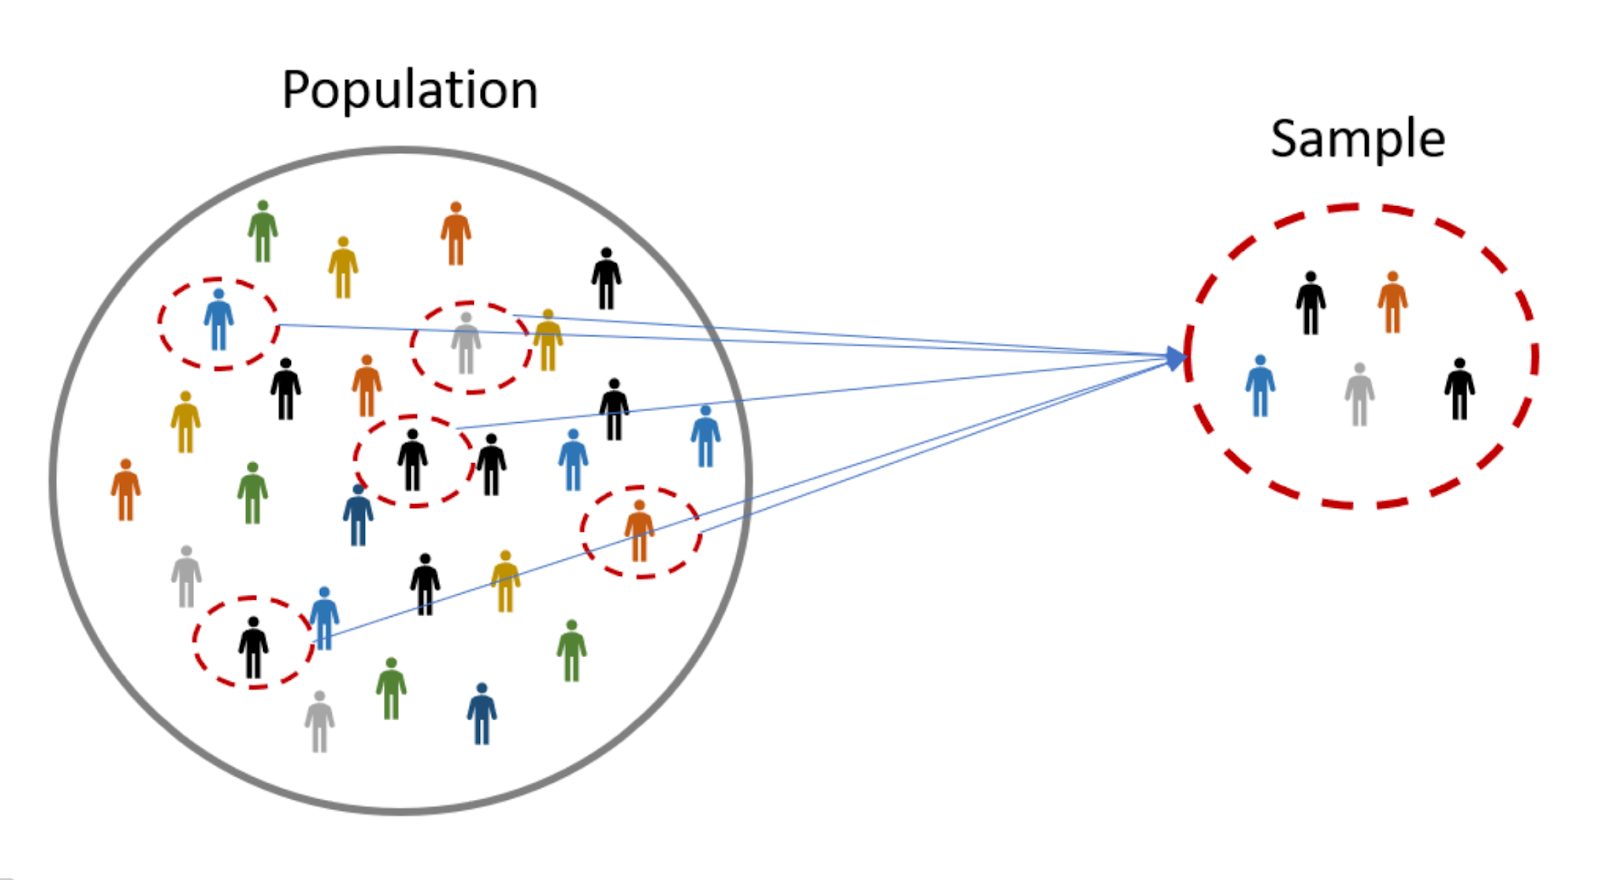
\includegraphics[width=0.9\textwidth]{/home/suzy/gitrepos/tuttelikz/machine-learning/221210-pca/images/sample_vs_population.png}
        \end{center}
    \end{frame}

    \subsection{Mean, standard deviation, variance}
    \begin{frame}
        \frametitle{Population vs sample}
        \begin{columns}
            \begin{column}{0.4\textwidth}  %%<--- here
                \begin{center}
                    \begin{block}{Population mean}
                        
                        \begin{equation}    % <--- deleted empty lines
                            \mu = \frac{\sum_{i=1}^N x_i}{N}
                        \end{equation}

                        $N$ is number of items in the population
                    \end{block}
                \end{center}
            \end{column}
            \begin{column}{0.4\textwidth}  %%<--- here
                \begin{center}
                    \begin{block}{Sample mean}
                        
                        \begin{equation}    % <--- deleted empty lines
                            \bar{{X}} = \frac{\sum_{i=1}^n x_i}{n}
                        \end{equation}
                        $n$ is number of items in the sample
                    \end{block}
                \end{center}
            \end{column}
        \end{columns}
    \end{frame}    
    
    \begin{frame}[fragile]
        \frametitle{Standard deviation}
        Let's take a look on two samples:\\~\\
        \begin{center}$A = \left[ 10\: 20\: 40\: 70 \right]$\end{center}
        \begin{center}
            
            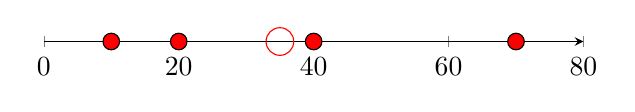
\begin{tikzpicture}
                \begin{axis}[
                    xmin=0, xmax=80,
                    axis x line=bottom,% only show the bottom x axis
                    hide y axis,    
                    ymin=0,ymax=1,
                    scatter/classes={%
                        a={mark=o,draw=black}}
                    ]
                
                \addplot[scatter,only marks,
                    mark size = 3pt,
                    fill = red,
                    scatter src=explicit symbolic]
                table {
                    10 0 
                    20 0 
                    40 0 
                    70 0 
                };
                \addplot[scatter,only marks,
                    mark size = 5pt,
                    mark=o,red,
                    scatter src=explicit symbolic]
                table {
                    35 0 
                };
                \end{axis}
                
            \end{tikzpicture}
        \end{center}
        
        \begin{center}$B = \left[ 30\: 33\: 37\: 40 \right]$\end{center}
        \begin{center}
            
            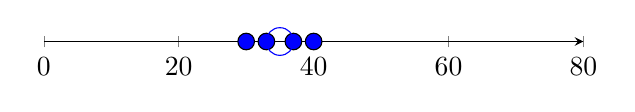
\begin{tikzpicture}
                \begin{axis}[
                    xmin=0, xmax=80,
                    axis x line=bottom,% only show the bottom x axis
                    hide y axis,    
                    ymin=0,ymax=1,
                    scatter/classes={%
                        a={mark=o,draw=black}}
                    ]
                
                \addplot[scatter,only marks,
                    mark size = 3pt,
                    fill = blue,
                    scatter src=explicit symbolic]
                table {
                    30 0 
                    33 0 
                    37 0 
                    40 0 
                };
                \addplot[scatter,only marks,
                    mark size = 5pt,
                    mark=o,blue,
                    scatter src=explicit symbolic]
                table {
                    35 0 
                };
                \end{axis}
                
            \end{tikzpicture}
        \end{center}
        Here, $\bar{{A}} = \bar{{B}} = 35$. Unfortunately, mean doesn't tell us a lot except for a middle point.
    \end{frame}

    \begin{frame}
        \frametitle{Standard deviation}
        For our two sets, $A = \left[ 10\: 20\: 40\: 70 \right]$ and $B = \left[ 30\: 33\: 37\: 40 \right]$, we would be more interested in the \emph{spread} of the data.
        \bigskip
        So, how do we calculate it?
        \begin{center}    
            \begin{block}{Standard deviation}
                \begin{equation}    % <--- deleted empty lines
                    s = \sqrt{\frac{\sum_{i=1}^n (X_i - \bar{X})^2}{(n-1)}}
                \end{equation}
                In plain English, it is the "average distance from the mean of the data set to a point."
            \end{block}
        \end{center}
        
    \end{frame}

    \begin{frame}[fragile]
        \frametitle{Standard deviation}
        Set 1: $A = \left[ 10\: 20\: 40\: 70 \right]$, and $\bar{A}=35$
        \begin{center}
            
            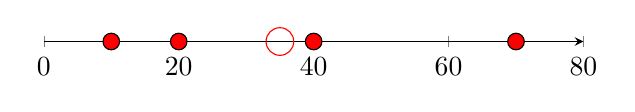
\begin{tikzpicture}
                \begin{axis}[
                    xmin=0, xmax=80,
                    axis x line=bottom,% only show the bottom x axis
                    hide y axis,    
                    ymin=0,ymax=1,
                    scatter/classes={%
                        a={mark=o,draw=black}}
                    ]
                
                \addplot[scatter,only marks,
                    mark size = 3pt,
                    fill = red,
                    scatter src=explicit symbolic]
                table {
                    10 0 
                    20 0 
                    40 0 
                    70 0 
                };
                \addplot[scatter,only marks,
                    mark size = 5pt,
                    mark=o,red,
                    scatter src=explicit symbolic]
                table {
                    35 0 
                };
                \end{axis}
                
            \end{tikzpicture}
        \end{center}
        Let's calculate standard deviation:
        \begin{center}
            \begin{tabular}{lrr}
                \firsthline
                $A$    & $(A-\bar{A})$ & $(A-\bar{A})^2$ \\
                \hline
                10      & -25    & 625      \\
                20        & -15        & 225       \\
                40       & 5     & 25      \\
                70       & 35     & 1,225      \\
                Total       &      &  2,100     \\
                Divided by (n-1)       &      & 700   \\
                Square root       &      & \textbf{26.4575}   \\
                \lasthline
                \end{tabular}
        \end{center}

    \end{frame}

    \begin{frame}[fragile]
        \frametitle{Standard deviation}
        Set 2: $B = \left[ 30\: 33\: 37\: 40 \right]$, and $\bar{B}=35$
        \begin{center}
            
            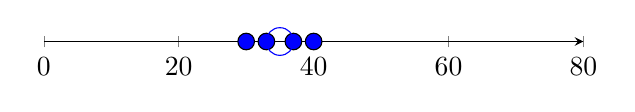
\begin{tikzpicture}
                \begin{axis}[
                    xmin=0, xmax=80,
                    axis x line=bottom,% only show the bottom x axis
                    hide y axis,    
                    ymin=0,ymax=1,
                    scatter/classes={%
                        a={mark=o,draw=black}}
                    ]
                
                \addplot[scatter,only marks,
                    mark size = 3pt,
                    fill = blue,
                    scatter src=explicit symbolic]
                table {
                    30 0 
                    33 0 
                    37 0 
                    40 0 
                };
                \addplot[scatter,only marks,
                    mark size = 5pt,
                    mark=o,blue,
                    scatter src=explicit symbolic]
                table {
                    35 0 
                };
                \end{axis}
                
            \end{tikzpicture}
        \end{center}
        Let's calculate standard deviation:
        \begin{center}
            \begin{tabular}{lrr}
                \firsthline
                $B$    & $(B-\bar{B})$ & $(B-\bar{B})^2$ \\
                \hline
                30      & -5    & 25      \\
                33        & -2        & 4       \\
                37       & 2     & 4      \\
                40       & 5     & 25      \\
                Total       &      & 58      \\
                Divided by (n-1)       &      & 19.333   \\
                Square root       &      & \textbf{4.397}   \\
                \lasthline
                \end{tabular}
        \end{center}
    \end{frame}

    \begin{frame}
        \frametitle{Variance}
        Similar to standard deviation
        \bigskip
        So, how do we calculate it?
        \begin{center}    
            \begin{block}{Variance}
                \begin{equation}    % <--- deleted empty lines
                    s^2 = \frac{\sum_{i=1}^n (X_i - \bar{X})^2}{(n-1)}
                \end{equation}
                Almost identical to the standard deviation (there is no square root in the formula).
            \end{block}
        \end{center}
    \end{frame}

    \subsection{Covariance, covariance matrix}
    \begin{frame}
        \frametitle{Covariance}
        Previous measures are 1-dimensional. How do we check relationship between the dimensions?
        \begin{center}    
            \begin{block}{Covariance}
                \textbf{Variance}
                \begin{equation}    % <--- deleted empty lines
                    var(X) = \frac{\sum_{i=1}^n (X_i - \bar{X})(X_i - \bar{X})}{(n-1)}
                \end{equation}
                \textbf{Covariance}
                \begin{equation}    % <--- deleted empty lines
                    covar(X,Y) = \frac{\sum_{i=1}^n (X_i - \bar{X})(Y_i - \bar{Y})}{(n-1)}
                \end{equation}
                How much dimensions vary from the mean \textit{with respect to each other}.
            \end{block}
        \end{center}
        \begin{itemize}
          \item Covariance between one dimension and itself gives variance.
        \end{itemize}
        
    \end{frame}

    \begin{frame}
        \frametitle{Covariance}
        \begin{center}
        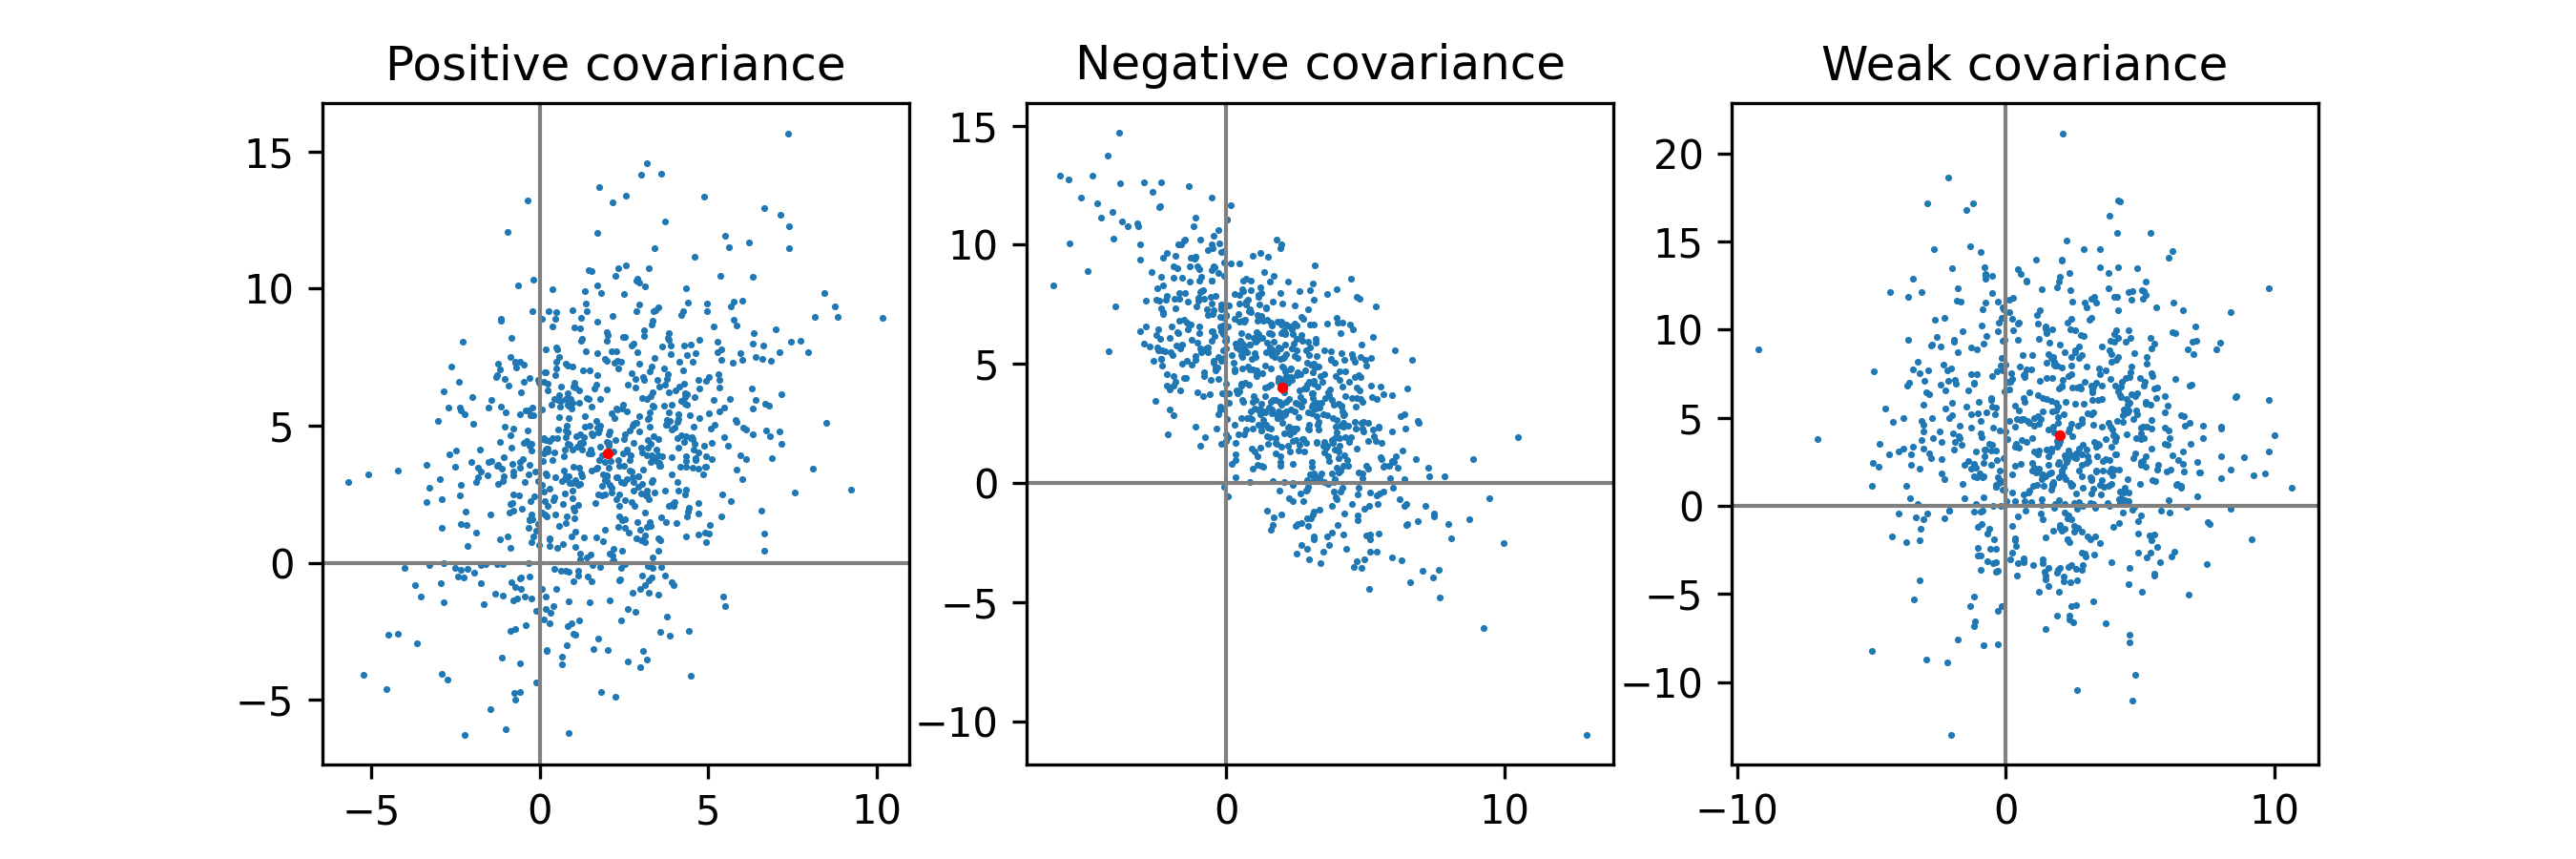
\includegraphics[width=1.0\textwidth]{/home/suzy/gitrepos/tuttelikz/machine-learning/221210-pca/images/covariance_types.png}
        \end{center}
    \end{frame}

    \begin{frame}
            \frametitle{Covariance}
            \underline{Exercise}: Find covariance between 2-dimensional dataset
            \begin{center}
                \begin{tabular}{ |c|c|c|c|c|c|c| } 
                \hline
                Item number: & 1 & 2 & 3 & 4 & 5 \\
                \hline
                x & 10  & 39 & 19 & 23 & 28 \\ 
                y & 43  & 13 & 32 & 21 & 20 \\ 
                \hline
                \end{tabular}
            \end{center} 
            \textbf{Ans: } -120.55
    \end{frame}

    \begin{frame}
        \frametitle{Covariance matrix}
        When we have more than two dimensions, covariances between individual dimensions could be described in covariance matrix\\
        
        \begin{center}    
            \begin{block}{Covariance matrix}
                \begin{equation}
                C^{n\times n} = (c_{i,j}: c_{i,j}=cov(Dim_{i}, Dim_{j}))
                \end{equation}
                where $C^{m\times n}$ is a matrix with $n$ rows and $m$ columns. Example for three dimensions:
                \begin{equation}    % <--- deleted empty lines
                    c = \begin{pmatrix}
                            cov(x,x) & cov(x,y) & cov(x,z)\\
                            cov(y,x) & cov(y,y) & cov(y,z)\\
                            cov(z,x) & cov(z,y) & cov(z,z)
                        \end{pmatrix}
                \end{equation}
                Since $cov(a,b) = cov(b,a)$, the matrix is symmetrical about the main diagonal. 
            \end{block}
        \end{center}
    \end{frame}

    \begin{frame}
        \frametitle{Covariance matrix}        
        \underline{Exercise}:  Find covariance matrix for the 3-dimensional dataset
        \begin{center}
            \begin{tabular}{ |c|c|c|c|c| } 
            \hline
            Item number: & 1 & 2 & 3 \\
            \hline
            x & 1  & -1 & 4 \\ 
            y & 2  & 1 & 3 \\ 
            z & 1  & 3 & -1 \\ 
            \hline
            \end{tabular}
        \end{center}
        \textbf{Ans: } $\begin{pmatrix}
            4.222 & 1.667 & -3.333 \\
            1.667 & 0.667 & -1.333 \\
            -3.333 & -1.333 & 2.667
        \end{pmatrix}$
\end{frame}


    \subsection{Eigenvectors, eigenvalues}
    \begin{frame}
        \frametitle{Eigenvectors}
        \begin{center}
            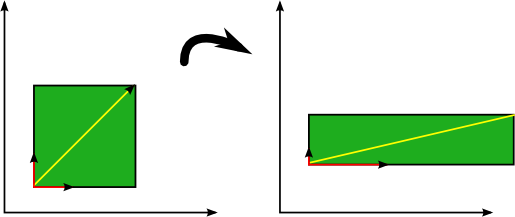
\includegraphics[width=0.7\textwidth]{/home/suzy/gitrepos/tuttelikz/machine-learning/221210-pca/images/eigenvectors.png}
        \end{center}
        %\vspace{0.5cm}
        \begin{itemize}
          \item Eigenvectors (red) do not change direction when a linear transformation (e.g. scaling) is applied to them. Other vectors (yellow) do.
        \end{itemize}
    \end{frame}

    \begin{frame}
        \frametitle{Eigenvectors}
        An example of non-eigenvector:
        \begin{equation}    % <--- deleted empty lines
            \colorlet{oldcolor}{black}
            \begin{pmatrix} 2 & 3 \\ 2 & 1 \end{pmatrix} \times \color{red} \boxed{\color{oldcolor} \begin{pmatrix} 1 \\ 3 \end{pmatrix} } \color{oldcolor} = \begin{pmatrix} 11 \\ 5 \end{pmatrix}
        \end{equation}

        An example of eigenvector:
        \begin{equation}    % <--- deleted empty lines
            \colorlet{oldcolor}{black}
            \begin{pmatrix} 2 & 3 \\ 2 & 1 \end{pmatrix} \times \color{blue} \boxed{\color{oldcolor} \begin{pmatrix} 3 \\ 2 \end{pmatrix} } \color{oldcolor} = \begin{pmatrix} 12 \\ 8 \end{pmatrix} = 4 \times \begin{pmatrix} 3 \\ 2 \end{pmatrix}
        \end{equation}

    \end{frame}

    \begin{frame}
        \frametitle{Eigenvalues}
        The amount by which the original vector was scaled after multiplication by the square matrix
        \begin{equation}    % <--- deleted empty lines
            \colorlet{oldcolor}{black}
            \begin{pmatrix} 2 & 3 \\ 2 & 1 \end{pmatrix} \times   \begin{pmatrix} 3 \\ 2 \end{pmatrix} = \begin{pmatrix} 12 \\ 8 \end{pmatrix} = \color{blue} \boxed{\color{oldcolor} 4} \color{oldcolor} \times \begin{pmatrix} 3 \\ 2 \end{pmatrix}
        \end{equation}
    \end{frame}

    \section{Dimensionality reduction techniques}
    \subsection{PCA (Principal component analysis)}
    \begin{frame}
        \frametitle{PCA}
        
        \textbf{What is Principal Component Analysis?} \\
        A way of identifying patterns in data: by highlighting their similarities and differences
        
        \bigskip
        \textbf{Pros}
        \begin{itemize}
            \item Once patterns in the data, and you compress the data, ie. by reducing the number of dimensions, without much loss of information.
        \end{itemize}

        \textbf{Cons}
        \begin{itemize}
            \item Linear $\therefore$ difficult to unfold single ambiguous object really belongs in several disparate locations in the low-dimensional space.
        \end{itemize}
    \end{frame}


    \subsubsection{Example with IRIS dataset}
    \begin{frame}
        \frametitle{Iris flower dataset}
        \begin{center}
        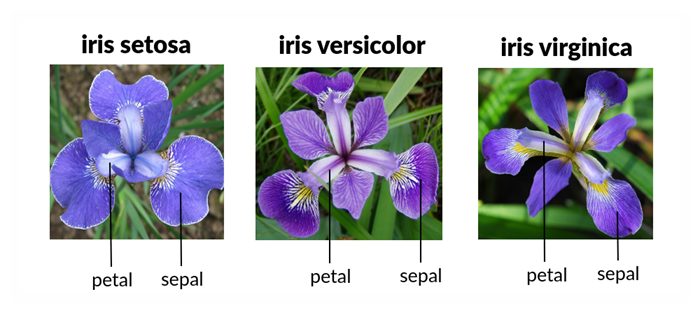
\includegraphics[width=0.9\textwidth]{/home/suzy/gitrepos/tuttelikz/machine-learning/221210-pca/images/iris.png}
        \end{center}
    \end{frame}
    
    \begin{frame}[fragile]
        \frametitle{Iris flower dataset}
        \begin{center}
        \begin{tikzpicture}[scale=0.8]
            \begin{axis}[width=6cm,height=6cm, xlabel = {Sepal length}, ylabel = {Sepal width}]
                \addplot+[scatter, only marks, scatter/classes={
                    Setosa={mark=square,red},
                    Versicolor={mark=triangle,green},
                    Virginica={mark=o,blue}}, scatter src=explicit symbolic] table[col sep=comma, header=true, x index=0, y index=1, meta index=4] {iris.csv};
                \legend{Setosa,Versicolor,Virginica},
            \end{axis}
        \end{tikzpicture}
        \hspace{1cm}
        \begin{tikzpicture}[scale=0.8]
            \begin{axis}[width=6cm,height=6cm, xlabel = {Petal length}, ylabel = {Petal width}]
                \addplot+[scatter, only marks, scatter/classes={
                    Setosa={mark=square,red},
                    Versicolor={mark=triangle,green},
                    Virginica={mark=o,blue}}, scatter src=explicit symbolic] table[col sep=comma, header=true, x index=2, y index=3, meta index=4] {iris.csv};
                \legend{Setosa,Versicolor,Virginica},
            \end{axis}
        \end{tikzpicture}
        \end{center}
        
    \end{frame}

    \begin{frame}
        \begin{center}
        \frametitle{Iris flower dataset}
        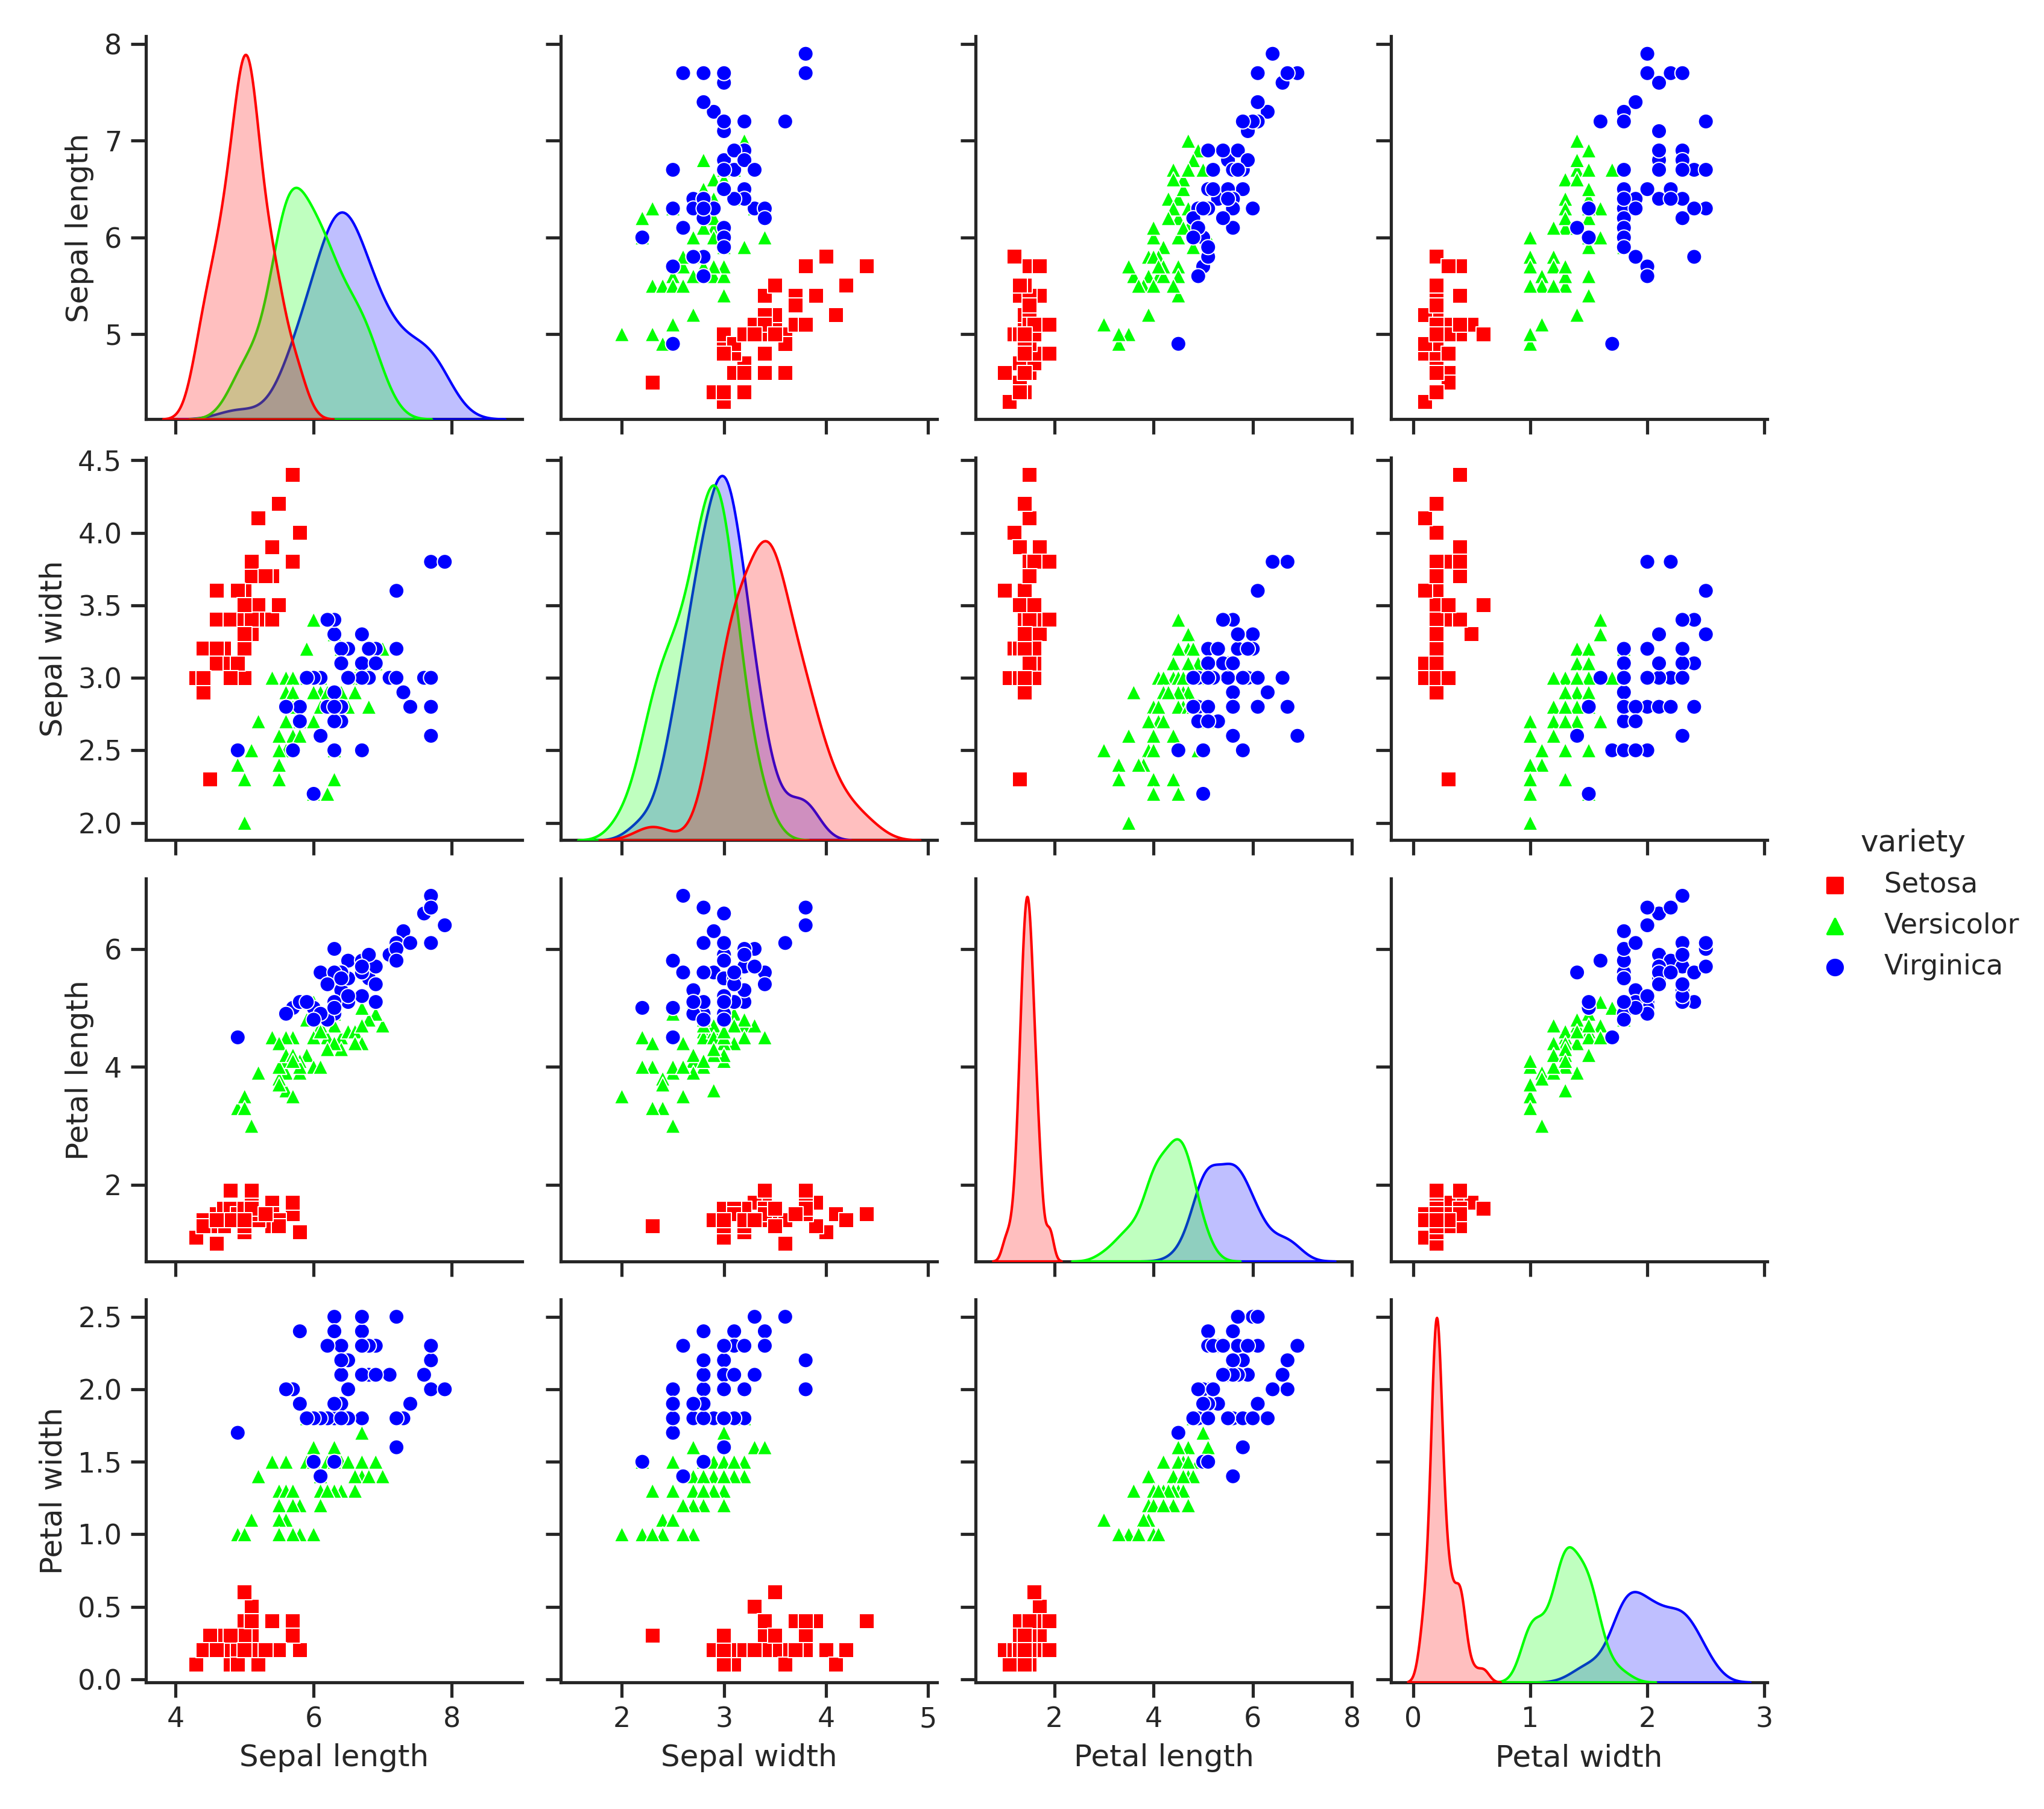
\includegraphics[width=0.7\textwidth]{/home/suzy/gitrepos/tuttelikz/machine-learning/221210-pca/images/pairplot_iris.png}
        \end{center}
    \end{frame}

    \begin{frame}[fragile]
        \frametitle{Applying PCA to Iris flower dataset}
        PCA automatically finds principal components (eg. \textit{axes}) in feature space. Here, we defined two, so we can visualize in 2D easily.
        \begin{columns}
            \begin{column}{0.5\textwidth}
                \scriptsize
                \begin{minted}[framesep=4mm, autogobble]{python}
                from sklearn import datasets
                from sklearn.decomposition import PCA

                iris = datasets.load_iris()

                X = iris.data
                y = iris.target
                target_names = iris.target_names

                pca = PCA(n_components=2)
                X_r = pca.fit(X).transform(X)
                \end{minted}
            \end{column}
            \begin{column}{0.5\textwidth}  %%<--- here
                \begin{center}
                    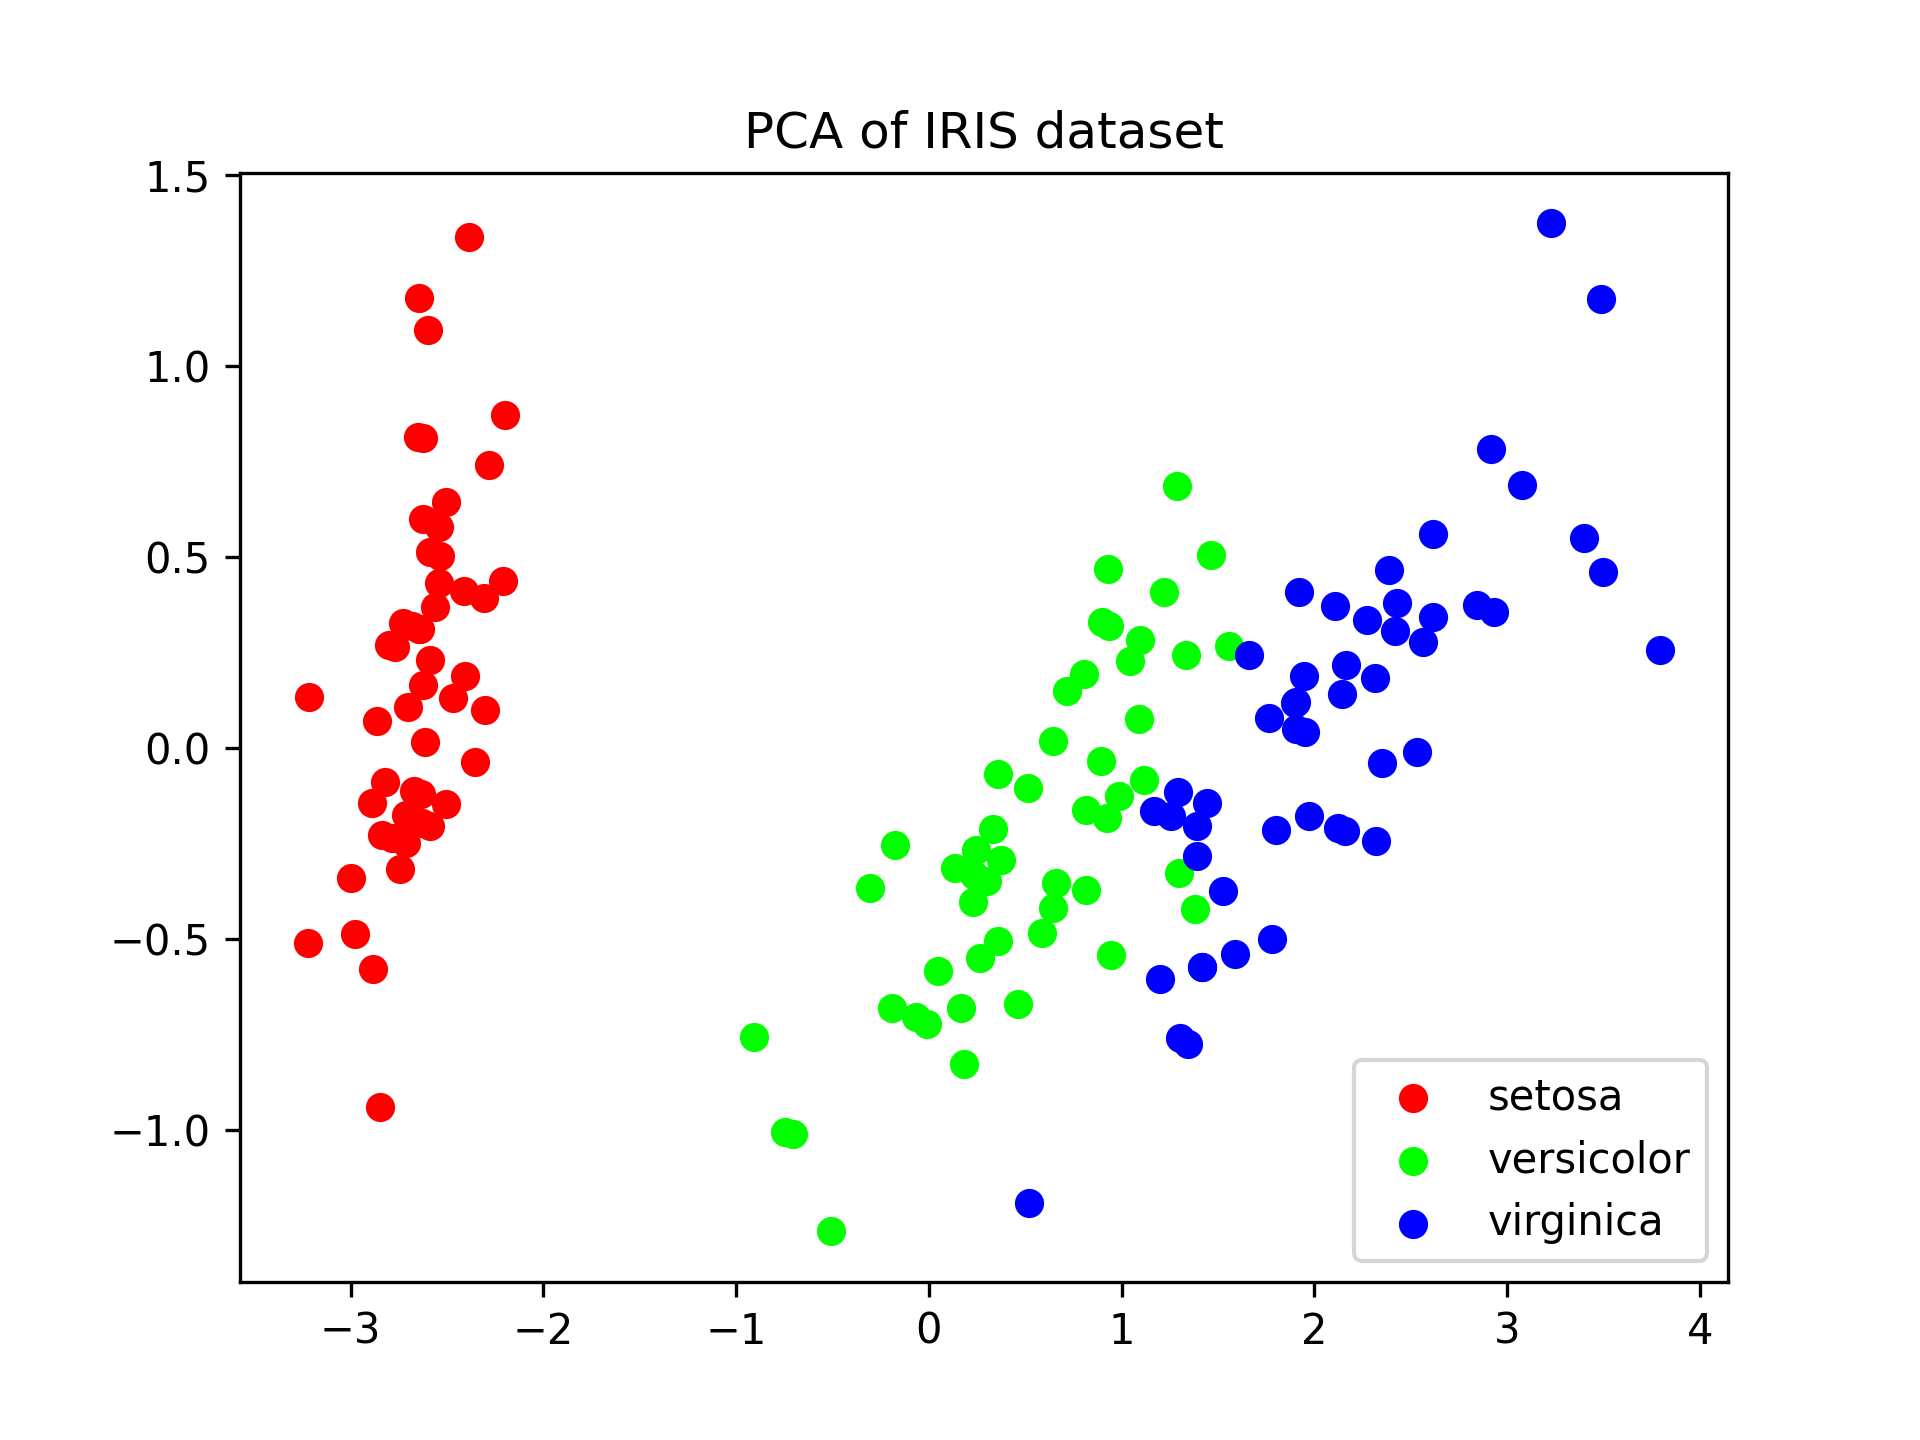
\includegraphics[width=1.0\textwidth]{/home/suzy/gitrepos/tuttelikz/machine-learning/221210-pca/images/pca_iris.png}
                 \end{center}
            \end{column}
        \end{columns}
    \end{frame}

    \subsubsection{PCA under the hood}
    \begin{frame}
        \begin{center}
        \frametitle{PCA under the hood}
        \resizebox{1.0\textwidth}{!}{
            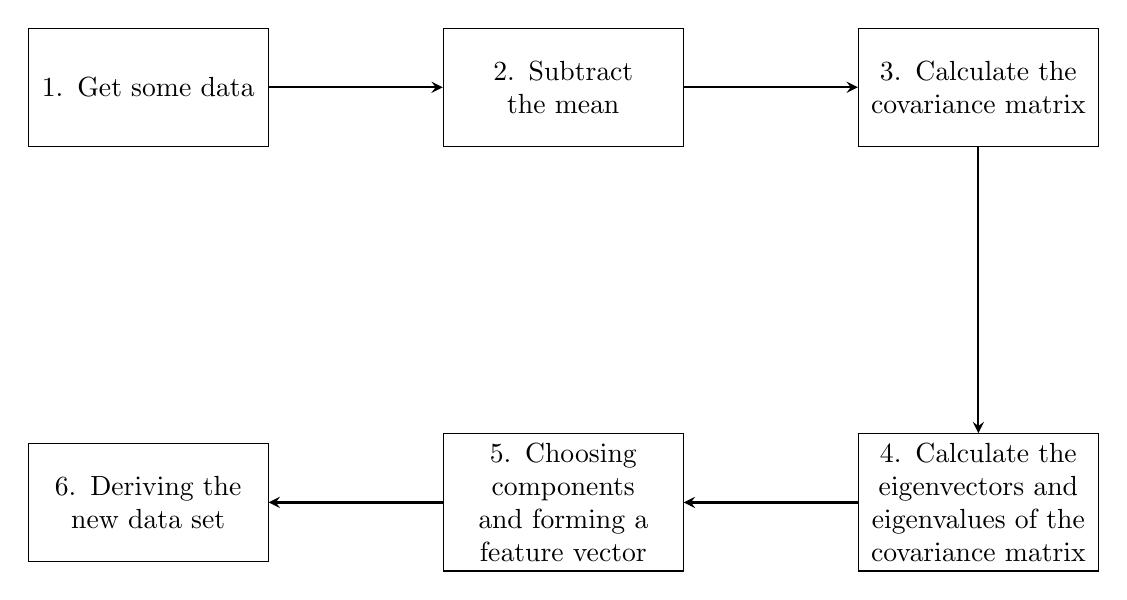
\begin{tikzpicture}
                % Create Blocks
                
                \node [block] (step2) {2. Subtract the mean};
                \node [block, left of=step2, xshift=-5em] (step1) {1. Get some data};
                \node [block, right of=step2, xshift=5em] (step3) {3. Calculate the covariance matrix};

                \node [block, below of=step3, yshift=-5em] (step4) {4. Calculate the eigenvectors and eigenvalues of the covariance matrix};
                \node [block, below of=step2, yshift=-5em] (step5) {5. Choosing components and forming a feature vector};
                \node [block, below of=step1, yshift=-5em] (step6) {6. Deriving the new data set};
                
                % Add Arrows
                \path [line] (step1) -- (step2);
                \path [line] (step2) -- (step3);
                \path [line] (step3) -- (step4);
                \path [line] (step4) -- (step5);
                \path [line] (step5) -- (step6);
            \end{tikzpicture}
        }
        \end{center}
    \end{frame}

    \begin{frame}[fragile]
        \frametitle{PCA under the hood}
        \begin{center}
        \scriptsize
        \begin{minted}[framesep=4mm, autogobble]{python}
        import numpy as np
        from numpy.linalg import eig

        def PCA_numpy(X,y):
            def mean(x): # np.mean(X, axis = 0)  
                return sum(x)/len(x)  

            def std(x): # np.std(X, axis = 0)
                return (sum((i - mean(x))**2 for i in x)/len(x))**0.5

            def Standardize_data(X):
                return (X - mean(X))/std(X)

            def covariance(x): 
                return (x.T @ x)/(x.shape[0]-1)

            # Step 1: Standardize the data
            X_std = Standardize_data(X)
            # Step 2: Find the covariance matrix
            cov_mat = covariance(X_std) # np.cov(X_std.T)

            # Step 3: Find the eigenvectors and eigenvalues of the covariance matrix
            eig_vals, eig_vecs = eig(cov_mat) 

        \end{minted}
        \end{center}
    \end{frame}

    \begin{frame}[fragile]
        \frametitle{PCA under the hood}
        \begin{center}
        \scriptsize
        \begin{minted}[framesep=4mm, autogobble]{python}
            max_abs_idx = np.argmax(np.abs(eig_vecs), axis=0)
            signs = np.sign(eig_vecs[max_abs_idx, range(eig_vecs.shape[0])])
            eig_vecs = eig_vecs*signs[np.newaxis,:]
            eig_vecs = eig_vecs.T

            # Step 4: Rearrange the eigenvectors and eigenvalues 
            eig_pairs = [(np.abs(eig_vals[i]), eig_vecs[i,:]) for i in range(len(eig_vals))]

            # Then, we sort the tuples from the highest to the lowest based on eigenvalues magnitude
            eig_pairs.sort(key=lambda x: x[0], reverse=True)
            eig_vals_sorted = np.array([x[0] for x in eig_pairs])
            eig_vecs_sorted = np.array([x[1] for x in eig_pairs])
            
            # Step 5: Choose principal components
            k = 2
            W = eig_vecs_sorted[:k, :] # Projection matrix

            # Step 6: Project the data
            X_proj = X_std.dot(W.T)

            return X_proj
        \end{minted}
        \end{center}
    \end{frame}

    \begin{frame}
        \frametitle{PCA under the hood}
        \begin{center}
            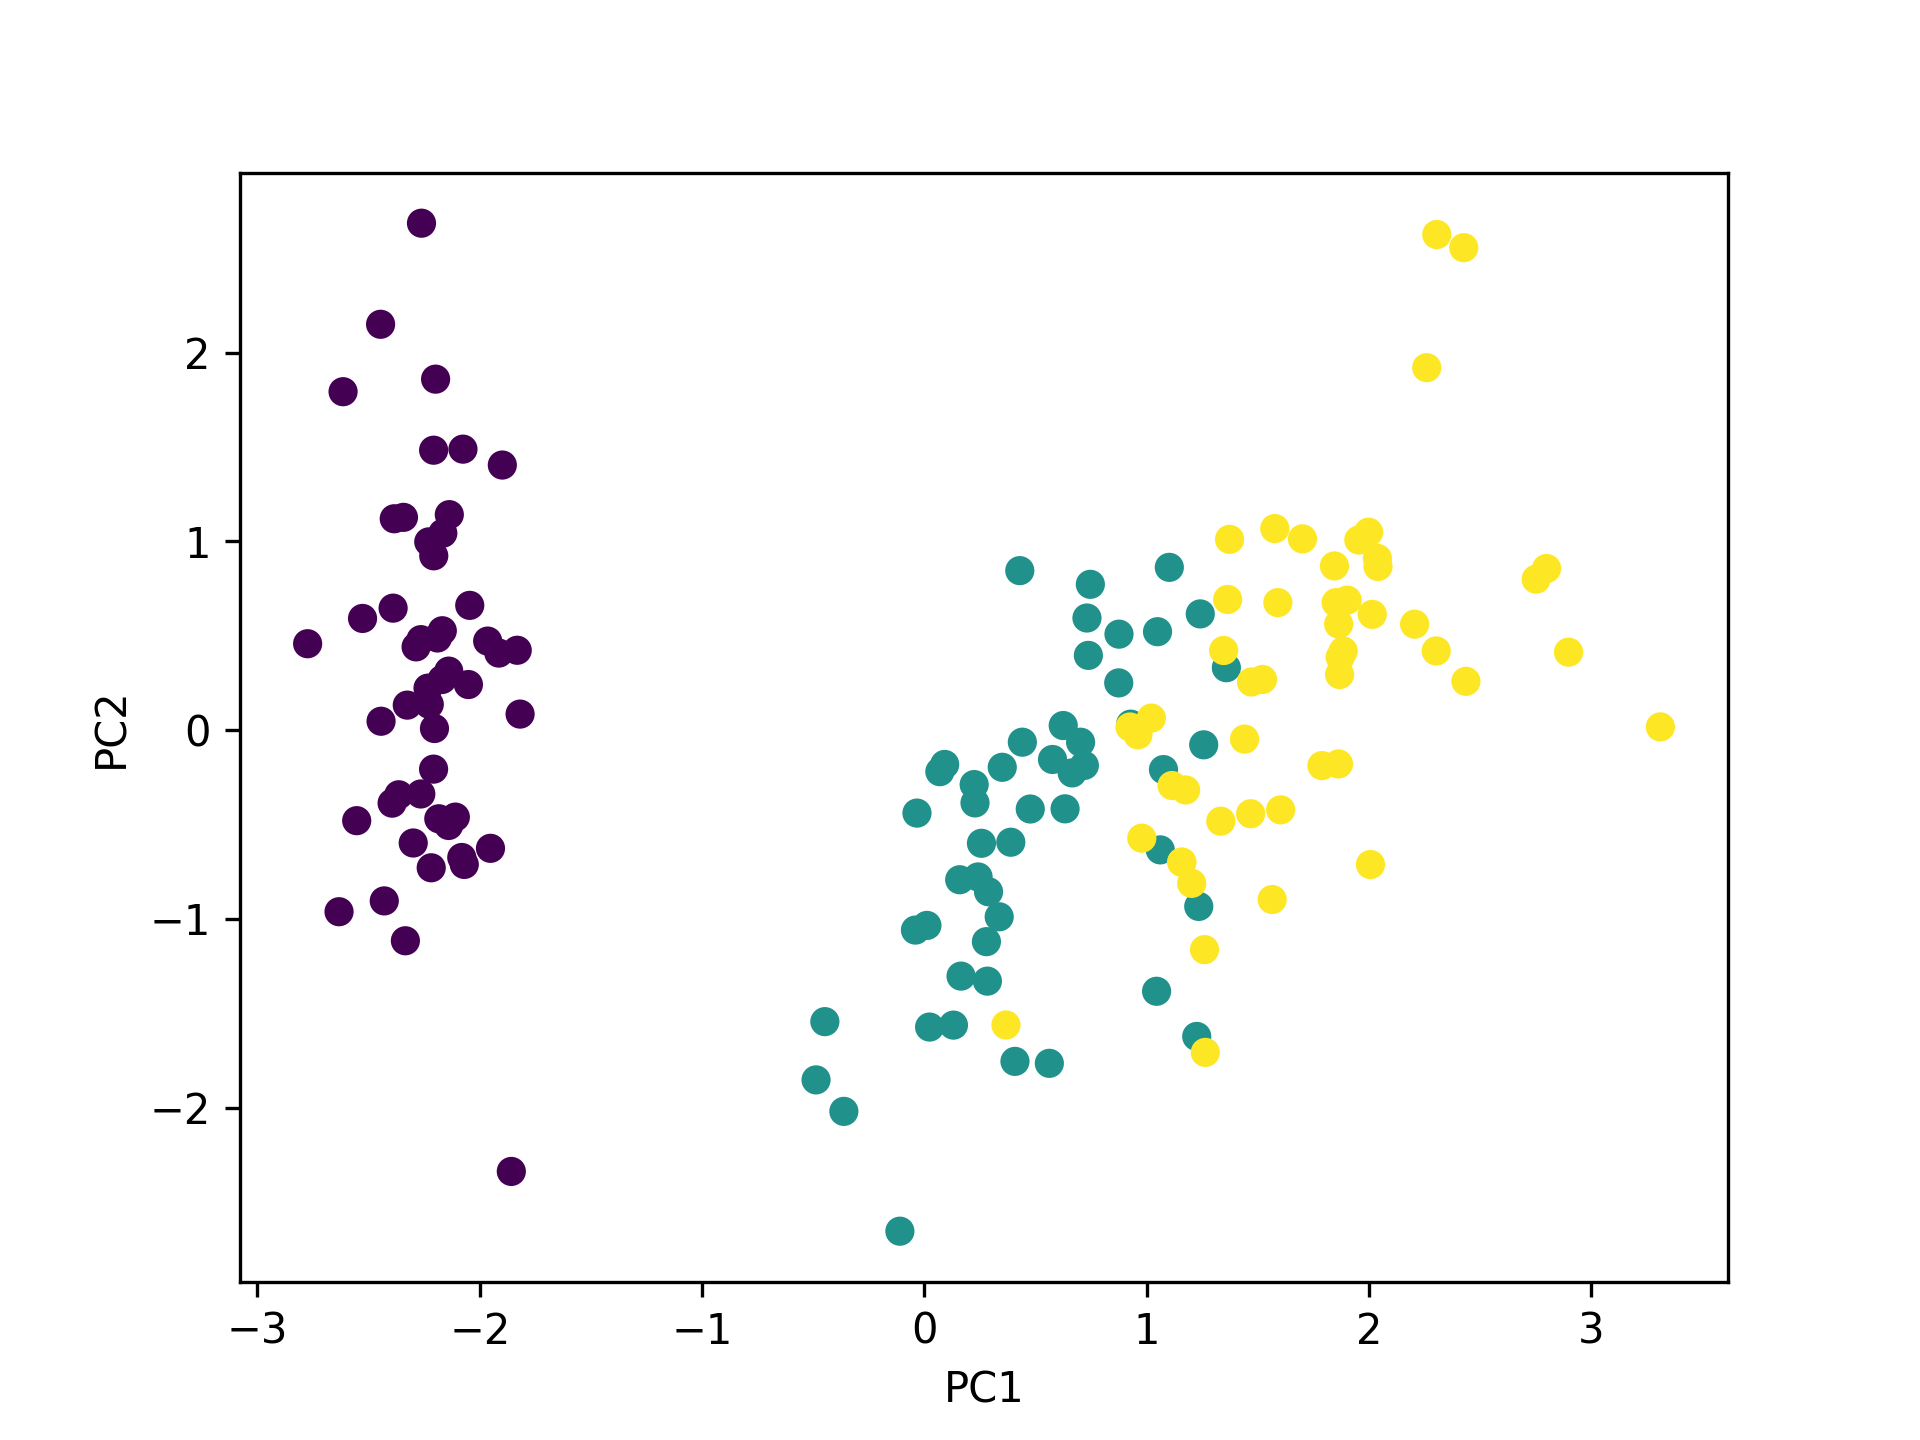
\includegraphics[width=0.9\textwidth]{/home/suzy/gitrepos/tuttelikz/machine-learning/221210-pca/images/pca_scratch.png}
        \end{center}
    \end{frame}

    \subsection{t-SNE (Stochastic neighbor embedding)}
    \begin{frame}
        \frametitle{t-SNE (Stochastic neighbor embedding)}
        \begin{center}
            To be continued
        \end{center}
    \end{frame}



    
    %mark=o,greenmark options={fill=red}

    \nocite{*}

    \section{Summary} %
    \subsection{Conclusion}
    \begin{frame}{Conclusion}

    \end{frame}


    \subsection{Practicum}
    \begin{frame}{Practicum}
      \begin{center}
      \begin{huge}Thank you for your attention!\end{huge}
      \end{center}

        % \vspace{0.5cm}
        % \begin{itemize}
        %   \item Workshop contents: \\
        %     \begin{small}\url{https://github.com/CodeSeoul/machine-learning/tree/master/221210-pca}
        %     \end{small}
        %   \item Follow-up QA? \\ 
        %     \begin{small}\url{http://discord.com/users/tuttelikz}
        %     \end{small}
        % \end{itemize}

    \end{frame}

    \begin{frame}{References}
      %\printbibliography  
    \end{frame}

\end{document}
